\section{Parallelization}
In this section we will describe a set of transformation rules known as Parallelizations. In \cref{fig:trivial-example} we use only the minimal number of modules necessary to produce the three recipes given in \cref{fig:toy-recipes}. It could easily be imagined that we had more modules capable of doing the same work as the ones in the given example. As such, we produce a set of transformation rules that allow for possibly greater throughput by parallelizing free modules with similar modules already in a line.


\subsection{$Para_0$: Parallelization Between Common Modules}
We start by defining the most common type of parallelization with the $Para_0$ transformation rule. Informally the rule states that if we have the total order $M_{s,e}$ of modules in between the modules $s$ and $e$. Then we can add a parallel line starting at $s$ and ending at $e$, if we can find an existing total order of free modules $P_{s,e}$ that can perform the same work as the modules in $M_{s,e}$. The visual representation of the $Para_0$ transformation rule can be seen \cref{fig:para0}. Here we expand the visual representation of our rules with the square box with a T in it. This box is just represents a single module that can perform no work, commonly referred to as a transport module.

\begin{figure}[H]
	\centering
	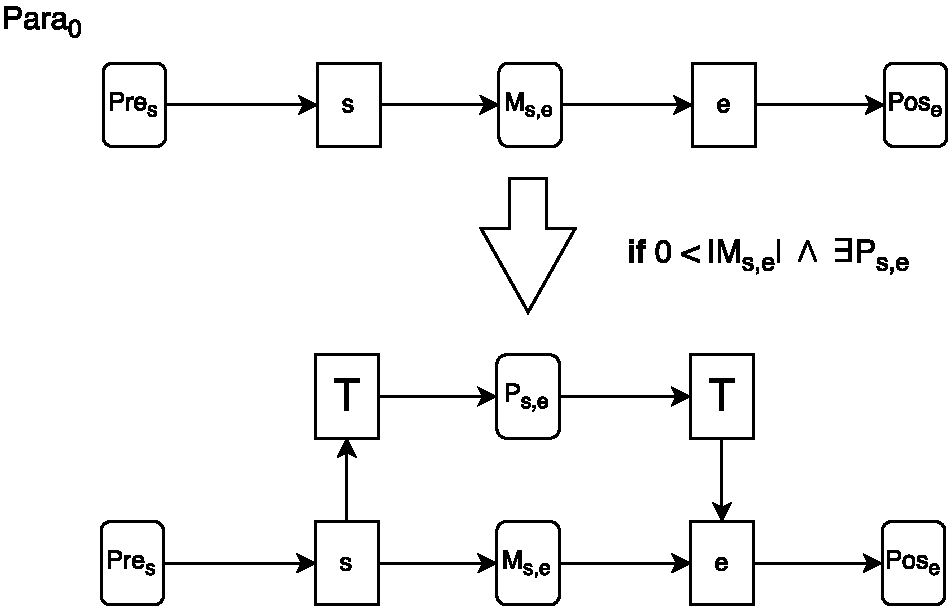
\includegraphics[width=0.7\textwidth]{para0.pdf}
	\caption{A visual representation of the $Para_0$ transformation rule}
	\label{fig:para0}
\end{figure}

In order to find the total order, $P_{s,e,}$, that can perform the same work as $M_{s,e}$. We first define the set of all free modules, $FM$. We say that the set of all free modules is the relative complement of all modules and all modules in a line $\gamma \in \Gamma$.

\[FM = M \setminus \{m | m \in \gamma \land \gamma \in \Gamma\}\]

We describe a set of pairs, where free modules are paired with modules in a total order $X$, if the free modules can at least do the same work as the work currently being done by the modules in $X$.

\[ParaMap_{X} = \{(m, m')| m \in FM \land m' \in X \land AW(m') \subseteq m\} \]

We then describe all sets of pairs that could be a possible parallel line for the modules in $X$. Note that this set could be the empty set, as the modules needed for creating a possible line might not available in $FM$.

\[ParaMapPaths_{X} = \{p \in ParaMap_{X}^2 | (m,m') \in p \land (n,n') \in p \land |p| = |X| \land  \forall m': m' \neq n' \}\]

After this we define $s[1]$ as the operation that given a set of pairs $s$, gives the set of all the first elements of the pairs in $s$.
\[s[1] = \{m_1 | (m_1, m_2) \in s\}\]

Using this we define the total order $P_{s,e}$ as:

\[ P_{s,e} = (p[1], \prec), \texttt{ where } p \in ParaMapPaths_{M_{s,e}} \]

This definition means that there might not exist any $P_{s,e}$ at all, or that there might be multiple candidates for $P_{s,e}$. Note that we replaced the set $X$ in $ParaMapPaths$ with the total order $M_{s,e}$.

Not shown in \cref{fig:para0} is that we also update the function $AW$ of our new configuration to $AW'$. We define $AW'$ as:

\[AW' = AW \cup p, \texttt{ where } p \in ParaMapPaths_
{M_{s,e}}\]

As with the rules for anti-serialization we also have two special cases for parallelization. Namely $para_1$, branch in, and $para_2$, branch out. The rest of this section will describe these two rules.

\subsection{$Para_1$: Branch in}
Again, similarly to $AS_1$, it may be that we wish to parallelize everything up to a certain module, without having branched out from some starting module. For this we describe the transformation rule $Para_1$, which can be seen in \cref{fig:para1}.

\begin{figure}[H]
	\centering
	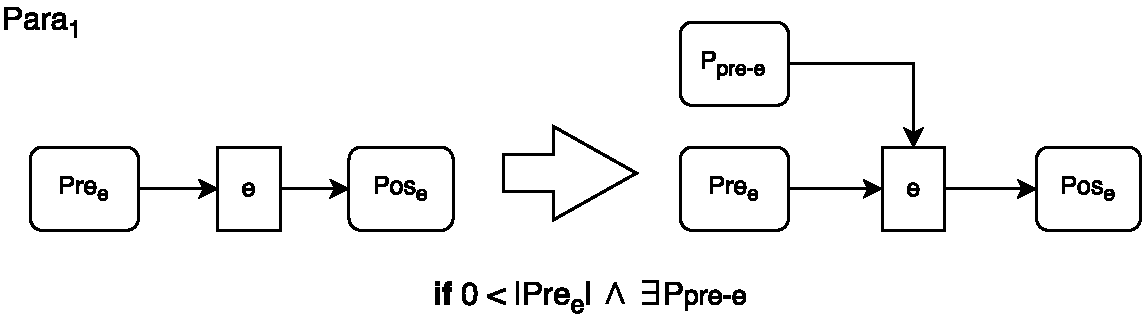
\includegraphics[width=0.8\textwidth]{para1.pdf}
	\caption{A visual representation of the $Para_1$ transformation rule}
	\label{fig:para1}
\end{figure}

We here define the total order as $P_{Pre_e}$ as:

\[P_{Pre_e} = (p[1], \prec), \texttt{ where } p \in ParaMapPaths_{Pre_e} \]

Not shown in \cref{fig:para1} is that we also update the function $AW$ of our new configuration to $AW'$. We define $AW'$ as:

\[AW' = AW \cup p, \texttt{ where } p \in ParaMapPaths_
{Pre_{s,e}}\]

\subsection{$Para_2$: Branch out}
We then, similarly to $AS_2$ describe the case in which we would like branch out parallelizing line, but not join it again. For this we describe the transformation rule $Para_2$, which can be seen in \cref{fig:para2}.

\begin{figure}[H]
	\centering
	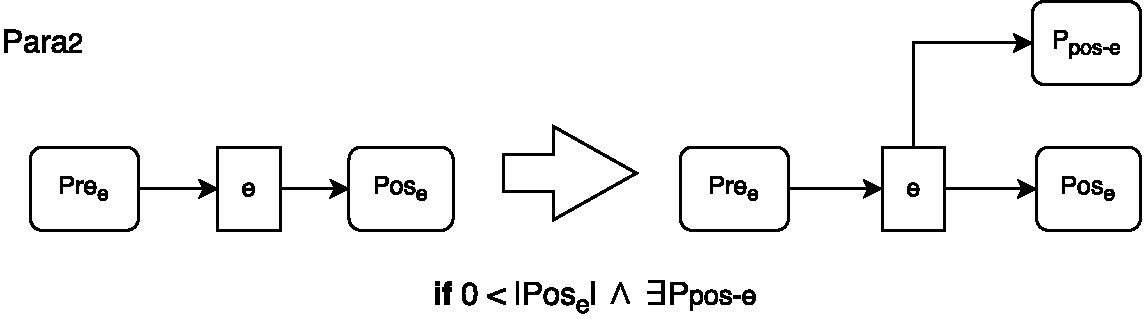
\includegraphics[width=0.8\textwidth]{para2.pdf}
	\caption{A visual representation of the $Para_2$ transformation rule}
	\label{fig:para2}
\end{figure}

We here define the total order $P_{Pos_e}$ as:

\[P_{Pos_e} = (p[1], \prec), \texttt{ where } p \in ParaMapPaths_{Pos_e} \]

Not shown in \cref{fig:para2} is that we also update the function $AW$ of our new configuration to $AW'$. We define $AW'$ as:

\[AW' = AW \cup p, \texttt{ where } p \in ParaMapPaths_
{Pos_{s,e}}\]


